\documentclass{article}

\usepackage{./qilinnotes}

\newcommand\Class{Grade 12 Chem}
\newcommand\Unit{Structure and Bonding}
\newcommand\Author{QiLin Xue}

\begin{document}
\maketitle

\tableofcontents
\newpage

\section{Quantum Mechanics}
\begin{itemize}
    \item Quantum theory is the product of several prior experiments. We shall explore a few of them to understand how we can utilize them to gain a fuller understanding of the atomic theory of matter. 
    \subsection{Quantization}
    \item Electrons can exist only at specific energy levels. Thus, it can only move between energy levels by either absorbing and emitting specific wavelengths of light. We can calculate the potential energy of electrons with different shells in hydrogen with the equation:
    $$
        E_n = -\frac{2.18\times 10^{-18} \text{ J}}{n^2}
    $$
    \item Johannes Rydberg developed an equation to describe the wavelength of light emitted from a specific electron transition in any atom:
    $$
        \frac{1}{\lambda} = RZ^2\left(\frac{1}{n^2_\text{lower}}-\frac{1}{n^2_\text{upper}}\right)
    $$
    \item When electricity is run through a gas, the gas tends to glow and emit light. This light can be separated using a prism. The sequence of wavelengths seen is called the \textbf{emission spectrum}. Similarly, light can be passed through a gas, and the gas will absorb only certain wavelengths. The resulting spectrum is called an \textbf{absorption spectrum}
    \subsection{Wave Particle Duality}
    \begin{review}
        All waves are defined by two defining features, the wavelength ($\lambda$) and the frequency ($\nu$). For light, these are related through the speed of light ($c=2.998 \times 10^8 \text{m/s}$):
        \begin{equation}
            \lambda = \frac{c}{\nu}
        \end{equation}
        and the energy is given by:
        \begin{equation}
            E = h\nu
        \end{equation}
        where $h = 6.6262 \times 10^{-34} \text{J}\cdot\text{s}$ is Planck's constant.
    \end{review}
    \item When any wave passes through a hole approximately as wide as their wavelength, the waves ``start over again," exhibiting a diffraction pattern.
    \item When there are two slits, waves can undergo constructive and destructive interference, as shown in the \textbf{Double Slit Experiment}. The surprising observation is that when electrons also exhibit the same behavior. This leads to the idea that matter and waves are interchangeable.
    \item The \textbf{de Broglie Wavelength} expresses the wavelength for any matter. We can relate wavelength and frequency to give an expression for energy:
    $$E = \frac{hc}{\lambda}$$
    Equating it with the mass-energy equivalence $E=mc^2$ we can generalize the speed of light to the speed of any matter. Replacing $mv$ with the momentum $p$, we can derive:
    \begin{equation}
        \lambda = \frac{h}{p}
    \end{equation}
    \begin{exampleQ}
        What is the de Broglie wavelength of an electron with mass $m=9.109 \times 10^{-31} \text{ kg}$ and speed $v = 2200 \text{ kms}^{-1}$?
    \end{exampleQ}
    \begin{exampleS}
        Using the de Broglie wavelength equation:
        $$\lambda = \frac{6.626 \times 10^{-34} \text{Js}}{(9.109 \times 10^{-31}\text{kg})(2200000 \text{m/s})} =  3.31 \times 10^{-10} \text{ m}$$
    \end{exampleS}
    \item When a wave is confined, under the right conditions, a \textit{standing wave} can be created. Electron waves can also exhibit this behavior as they are confined in a circle around an atom. The wider the radius, the more peaks it will have.
    \begin{center}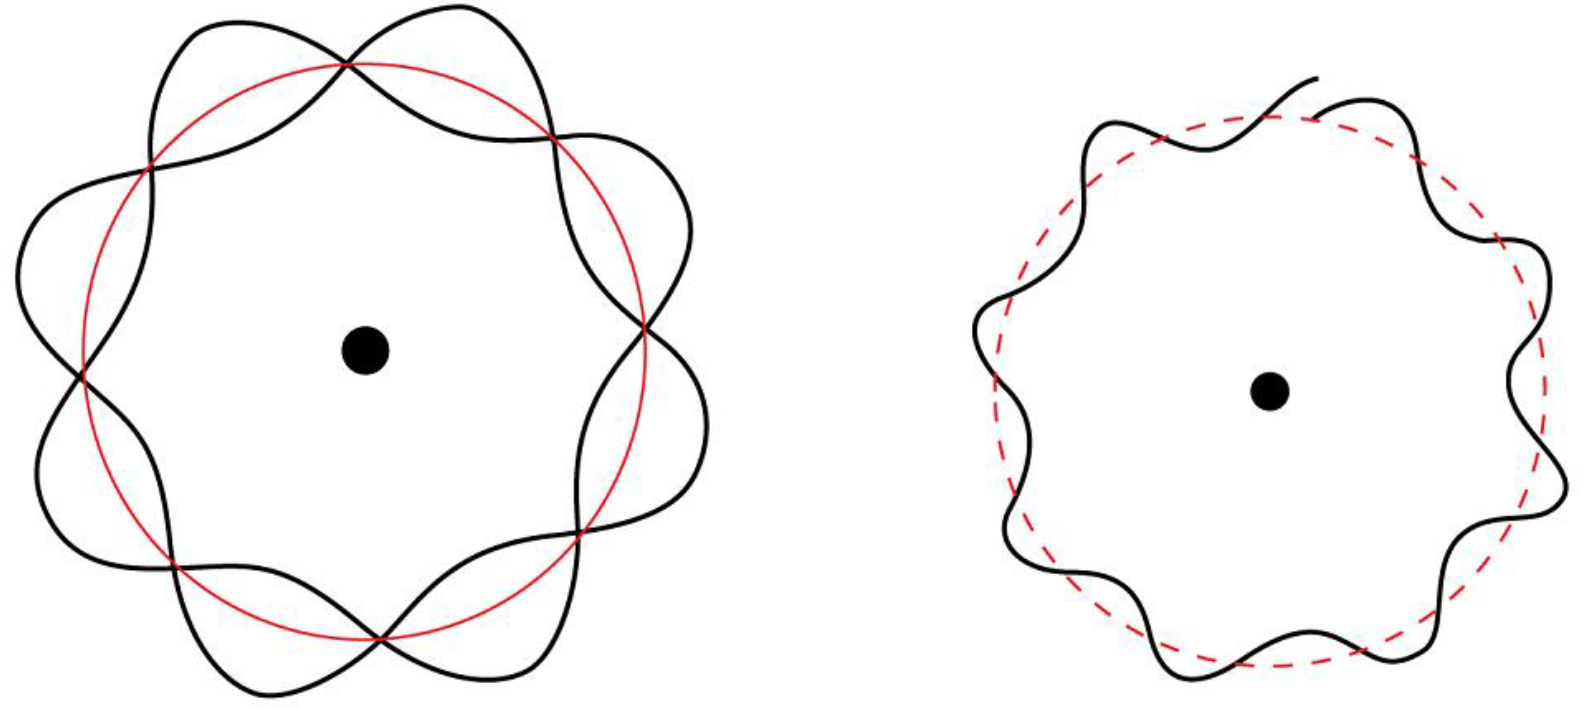
\includegraphics[width=0.5\linewidth]{Q1.PNG}\end{center}
    However, this can only accomplished with specific radii that offers the right interference patterns. Otherwise, resonance will not occur.
    \subsection{Quantum Numbers}
    \begin{idea}
        The standing waves are described by the time independent Schrodinger Wave Equation:
        $${\displaystyle \left[{\frac {-\hbar ^{2}}{2m}}\nabla ^{2}+V(\mathbf {r} )\right]\Psi (\mathbf {r} )=E\Psi (\mathbf {r} )}$$
        For a hydrogen atom, the solution is in terms of integer quantum numbers:
        $$\Psi(r,\theta,\phi) =  R(r)P(\theta)F(\phi)$$
        where the three factors correspond to the quantum numbers $n$, $l$, and $m_l$.
    \end{idea}
    \item The \textbf{principal quantum number} ($n$) is an integer number starting from $1$ that describes the energy level the electron is in.
    \item The \textbf{orbital quantum number} ($l$) describes the sub-shells in a given energy level the electron is in. They are represented by the digits $0,1,2,\cdots$ for $s$, $p$, $d$, $f$ subshells.
    \item The \textbf{magnetic quantum number} ($m_l$) describes which orbital the electron is in. The numbers are in the range $[-l,l]$ such that the middle orbital satisfies $m_l=0$.
    \begin{itemize}
        \item The first two quantum numbers are derived by observing electron jumps between shells and subshells in its emission spectrum. However, a magnetic field is able to separate electrons who were originally at the same energy level to different energy levels by changing the energy of the orbitals.
    \end{itemize}
    \item The \textbf{spin quantum number} ($m_s$) describes the spin of the electron. The two spin numbers are $+\frac{1}{2}$ (up) or $-\frac{1}{2}$ (down).
    \begin{itemize}
        \item Of course, the electrons are not actually spinning. The original reason early physicists thought they were spinning was due to the connection between spinning charges with magnetic fields. There is no simple physical intuition.
    \end{itemize}
    \subsection{Atomic Orbitals}
    \item There are four orbitals: $s$, $p$, $d$, and $f$ each able to hold two electrons.
    \item The $s$ orbital is modelled by a sphere
    \begin{center}
    \begin{tikzpicture}
        \orbital[pos = {(0,5.5)}]{s}
    \end{tikzpicture}
    \end{center}
    \item The $p$ orbital is modelled by two dumbbells:
    \begin{center}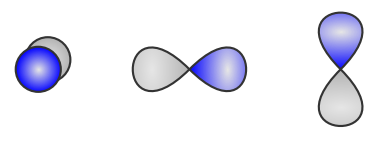
\includegraphics[width=0.3\linewidth]{Q3.PNG}\end{center}
    % \begin{center}
    % \begin{tikzpicture}
    %     \orbital[pos = {(0,3)}]{px}
    %     \node[above] at (0,4) {2p$_x$};
    %     \orbital[pos = {(2,3)}]{py}
    %     \node[above] at (2,4) {2p$_y$};
    %     \orbital[pos = {(4,3)}]{pz}
    %     \node[above] at (4,4) {2p$_z$};
    % \end{tikzpicture}
    % \end{center}
    \item The $d$ orbital is modelled by a clover:
    \begin{center}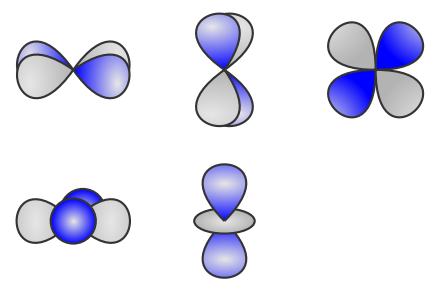
\includegraphics[width=0.3\linewidth]{Q4.PNG}\end{center}
    \item Higher energy levels ($2s$, $3p$, $4d$) and so on have layers within their orbitals.
    \begin{center}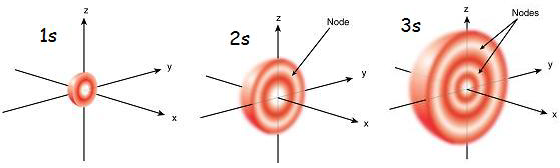
\includegraphics[width=0.6\linewidth]{Q5.PNG}\end{center}
    \item At the center of the nucleus, there is a zero probability of finding an electron there and it increases the farther away we get from the nucleus. For orbitals with higher energy levels, there be a nodal surface in the electron wave and it will start becoming more dense again.
    \subsection{Uncertainty}
    \begin{idea}
        The Heisenberg Uncertainty Principle states that the uncertainty of an objects position and momentum is related through the equation:
        \begin{equation}
            \Delta x \Delta p \ge \frac{h}{4\pi}
        \end{equation}
    \end{idea}
    \item The Copenhagen Interpretation is statistical based where each state is assigned a certain probability and that without being observed it exists in every state at once.
    \item Therefore, we need to refer to \textit{clouds of electron density} instead of definite paths for electrons
    \item We can graph their uncertainty with electron density graphs.
    \begin{center}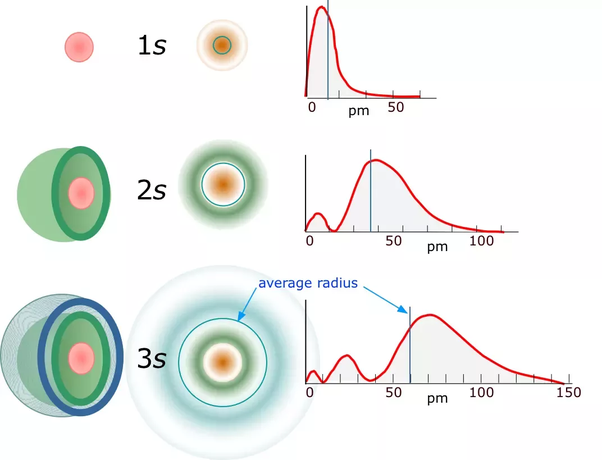
\includegraphics[width=0.5\linewidth]{Q2-TEMP.PNG}\end{center}
    \item Due to the probabilistic approach of viewing matter, every particle has a probability of existing anywhere. They don't physically traverse the space in between, hence called \textit{quantum tunnelling}. For example, neutrons and protons in a nucleus can occasionally pop out, resulting in \textbf{radioactive decay}.
    \subsection{Electron Configuration}
    \begin{review}
        There are three rules to determine how to place electrons in their orbitals.
        \begin{itemize}
            \item \textbf{Aufbau Principle} - Electrons fill atomic orbitals of the lowest available energy levels before occupying higher levels
            \item \textbf{Hund's Rule} - Every orbital in a subshell is singly occupied with one electron before any one orbital is doubly occupied.
            \item \textbf{Pauli Exclusion Principle} - No two electrons can have the same four quantum numbers.
        \end{itemize}
    \end{review}
    \item The electron configuration of an atom goes in order of the periodic table from lowest energy to highest:
    \begin{center}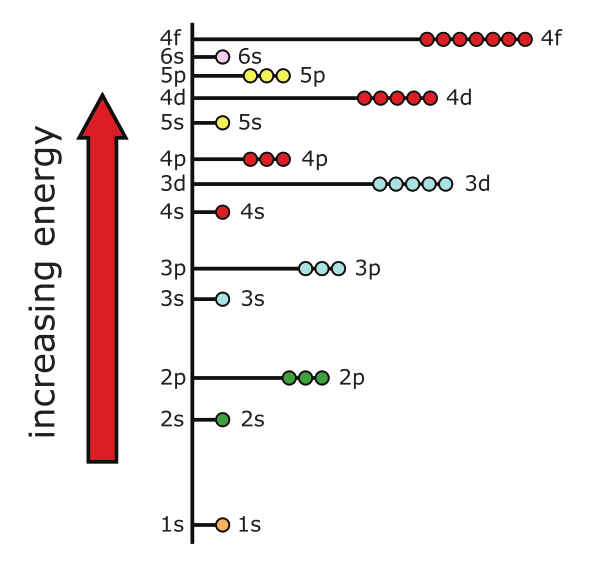
\includegraphics[width=0.3\linewidth]{Q6.PNG}\end{center}
    \item For example, iron has an electron configuration of
    $$\mathrm{1s^22s^22p^63s^23p^64s^23d^6}$$
    \item The shorthand form starts from the last noble gas. For iron, it would be:
    $$\mathrm{[Ar]4s^23d^6}$$
    \item Sometimes, if the $d$ orbital is one electron away from being full or half-full, an electron from the $s$ orbital may jump to the $d$ orbital. This is caused by the high repulsion in the $s$ orbital Since two electrons occupy the same orbital repelling each other. The $s$ orbital also overlaps with each of the $d$ orbitals, further increasing the repulsion felt. For example, the configuration for chromium is:
    $$\mathrm{[Ar]4s^13d^5}$$
    \item When electrons become ions, we remove or add the electron in the highest energy state. However: when removing electrons when the $p$ subshell is full or half-full, always remove the electrons from the $s$ orbital first. 
    \subsection{Ionization Energy and Electron Affinity}
    \item The \textit{ionization energy} describes the energy required to remove an electron. It is proportional to the force holding the electron in place.
    \begin{exampleQ}
        Why does aluminum have a lower ionization energy than expected (and lower than magnesium)?
    \end{exampleQ}
    \begin{exampleS}
        In the traditional sense of looking at the atom, the ionization energy is directly proportional to the effective nuclear charge and inversely proportional to the square of the distance away from the nucleus. Aluminum has an ENC of $3$ while magnesium has an ENC of $2$. We would expect this extra force to pull the valence electrons in aluminum inwards further increasing the force and increasing its ionization energy.\\

        However, we find that this is not the case. In the quantum model of the atom, the highest energy electron in aluminum is actually in the $3p$ subshell, which is farther away than the $3s$ subshell. The $3p$ subshell also overlaps with the electron density cloud defined by the $3s$ orbital. This added repulsion along with the further distance decreases the columbic force and makes it easier to remove it, resulting in a lower ionization energy.
    \end{exampleS}
    \item The \textit{electron affinity} refers to how strongly it can hold onto new electrons. It is equal to the energy released when a new electron is put into the orbit. A negative number means that it releases energy while a positive number means you have to do outside work to put it into the orbit (absorbs energy)
    \begin{exampleQ}
        Why do some elements (like $\mathrm{N}$ and $\mathrm{Mg}$) have electron affinities $\le 0$?
    \end{exampleQ}
    \begin{exampleS}
        The negative electron affinity tells us that we need to put energy into the system in order for a new electron to be added into the orbit. The electron configuration for nitrogen is $\mathrm{[He]2s^22p^3}$. Adding another electron would mean one $p$ orbital would contain two electrons and when two electrons occupy the same electron density cloud, it can increase repulsion forces. \\

        For magnesium, the electron configuration is $\mathrm{[Ne]3s^2}$. The next electron added would have to be in the $3p$ subshell, which not only is at a farther distance from the $3s$ subshell but overlaps with the $3s$ orbital a lot which creates a shielding effect. These two effects greatly reduce the columbic force the added electron feels so much that it actually repels nearby electrons.
    \end{exampleS}
\end{itemize}
\end{document}